\begin{frame}{Metodologia}
    \begin{itemize}
        \item Implementar malhas da superfície com tamanho pseudo-infinito;
        
    \end{itemize}
    
    \begin{figure}[H]
        \centering
        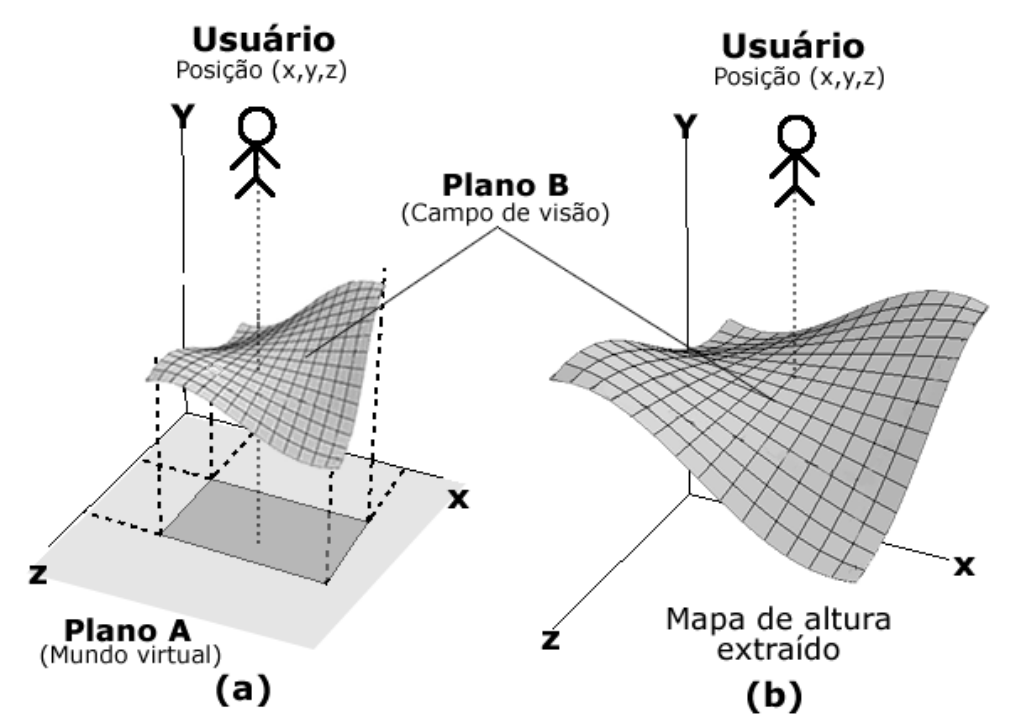
\includegraphics[width=.6\textwidth, height=.5\textheight]{img/malhaPInf}
        \caption{Exemplo de malha. Por \cite{bevilacquaferramenta}}
        \label{fig:malhaPInf}
    \end{figure}
    
    
    
\end{frame}

\begin{frame}{Metodologia}
    \begin{itemize}
        \item Selecionar biomas, e as características dos mesmos a ser representadas;
        \item Construir algoritmo para manipular ruído de Perlin e gerar características
            selecionadas do bioma;
    \end{itemize}
    \begin{figure}
        \centering
        \begin{subfigure}[b]{0.47\textwidth}
            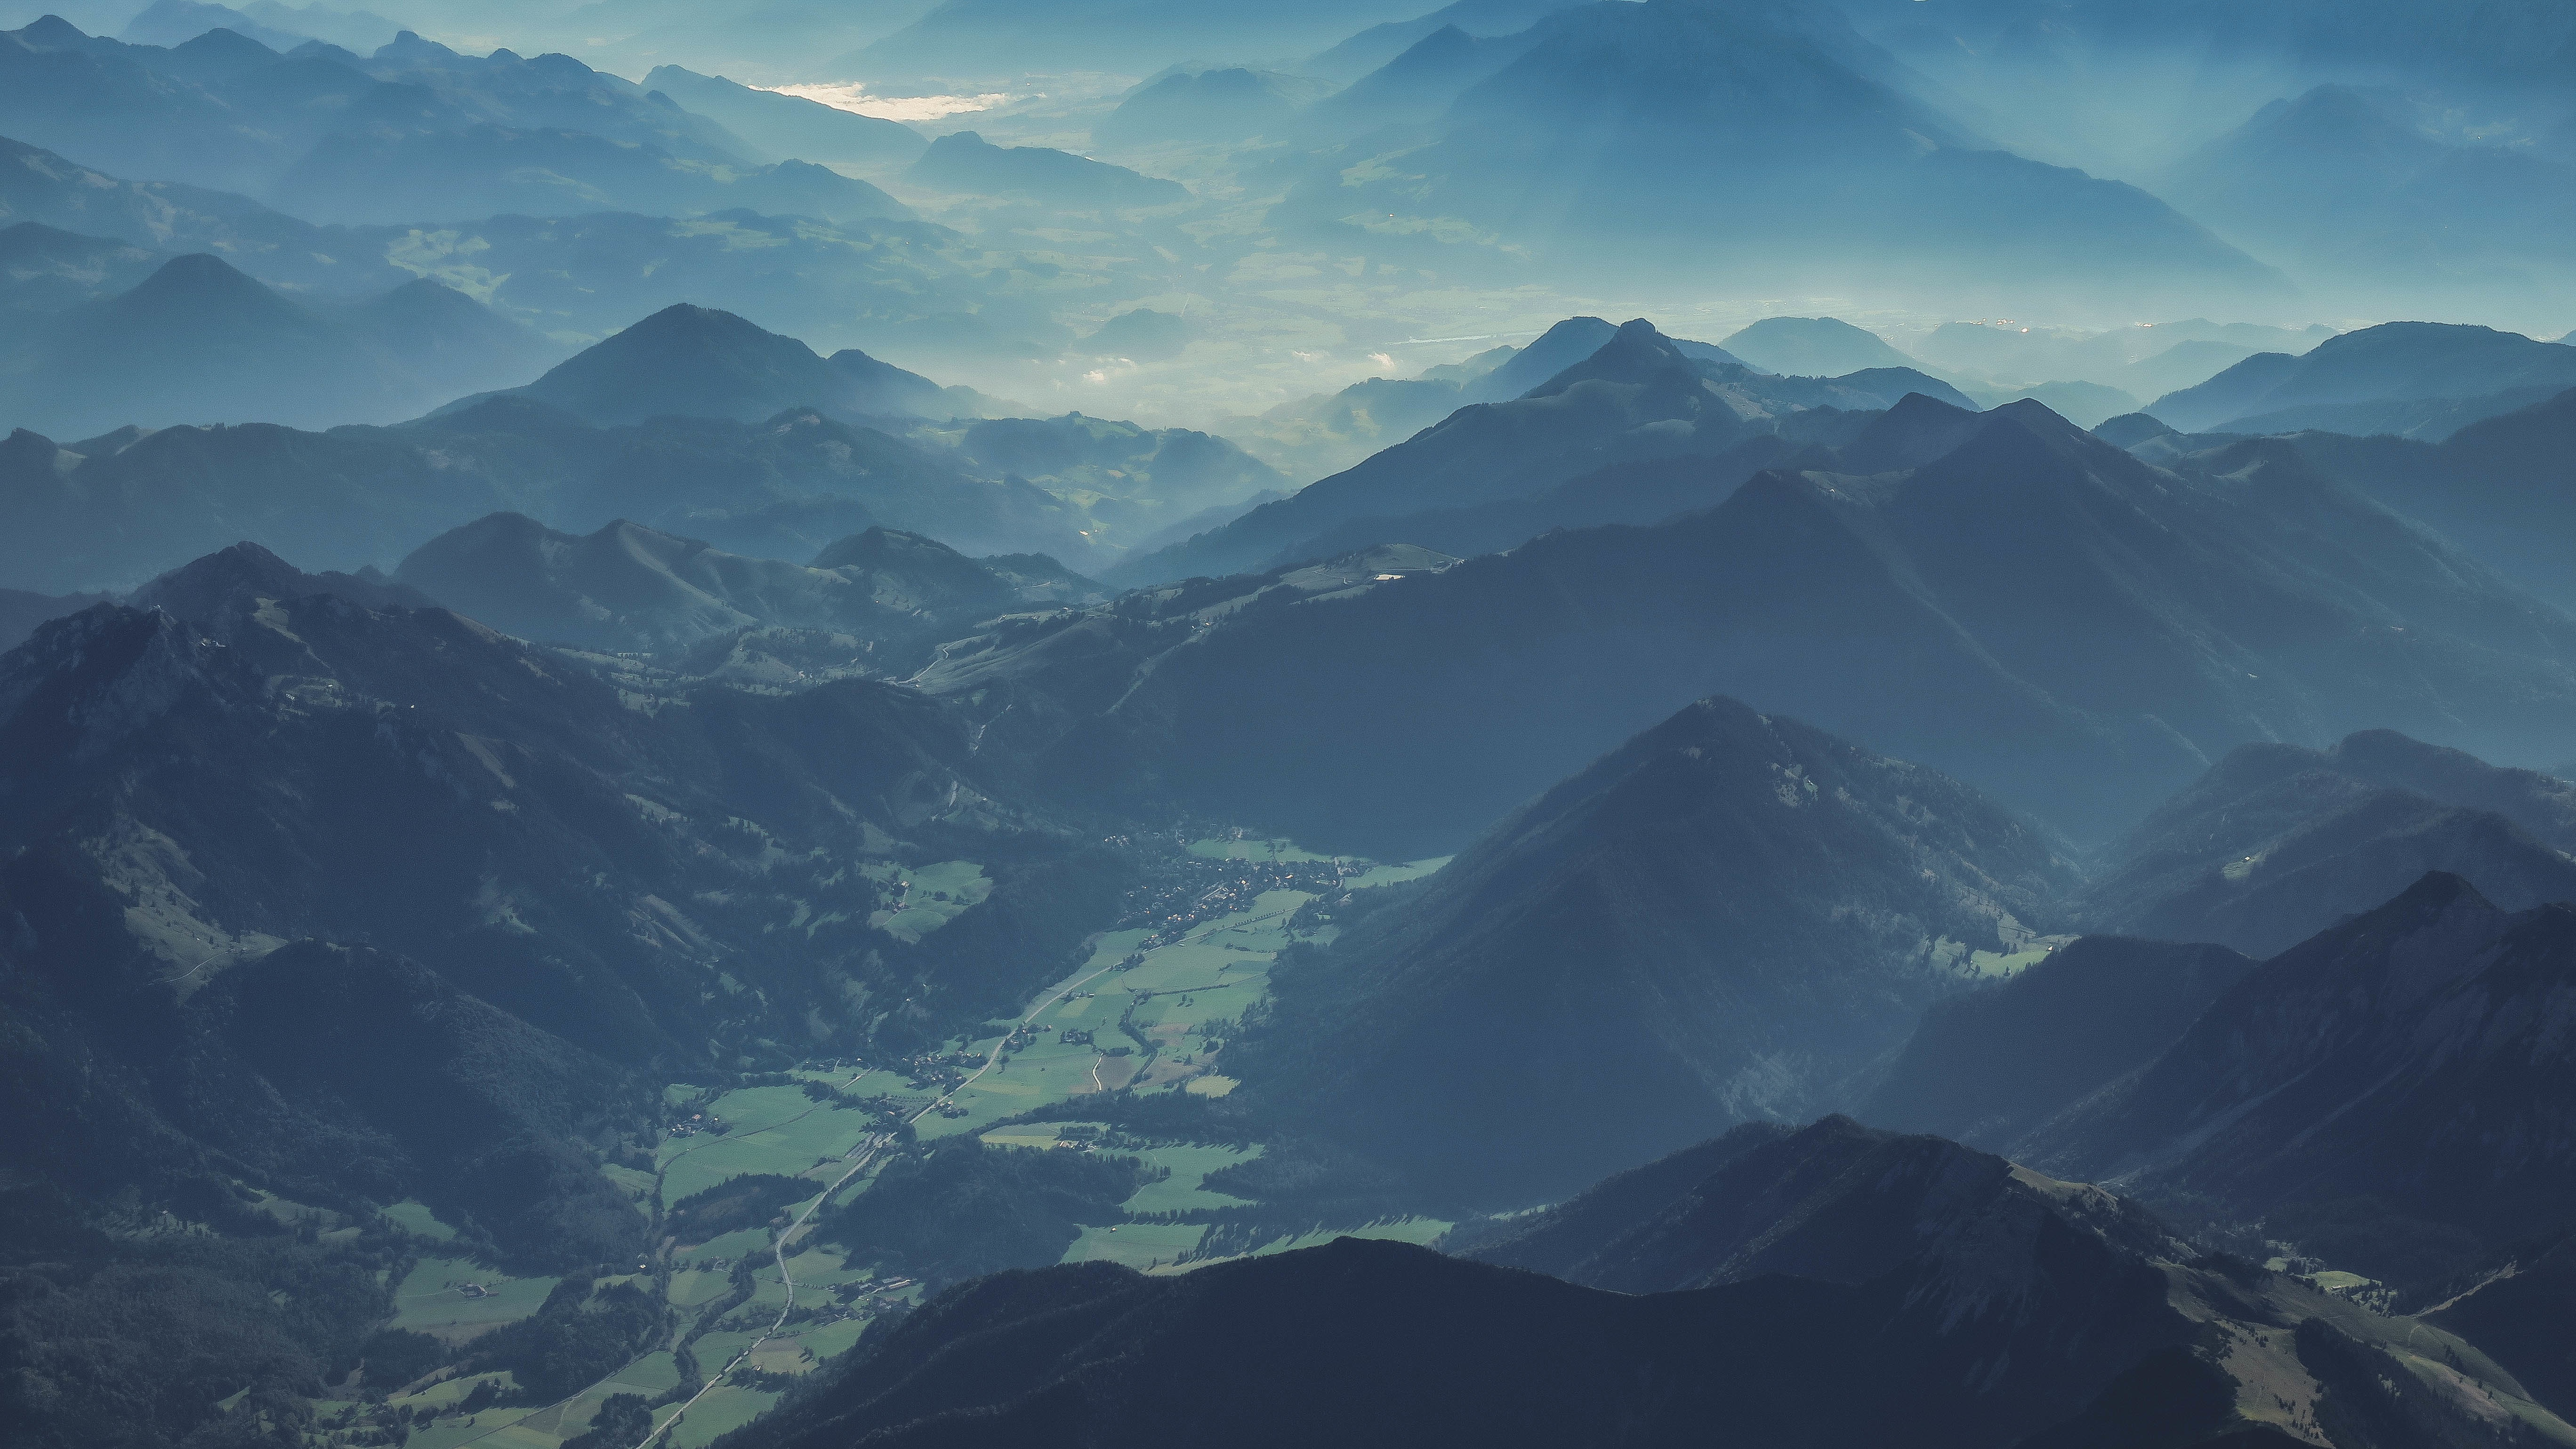
\includegraphics[width=\textwidth]{img/mountains}
            \caption{Cordilheiras}
            \label{fig:mountains}
        \end{subfigure}
        ~ %add desired spacing between images, e. g. ~, \quad, \qquad, \hfill etc. 
          %(or a blank line to force the subfigure onto a new line)
        \begin{subfigure}[b]{0.47\textwidth}
            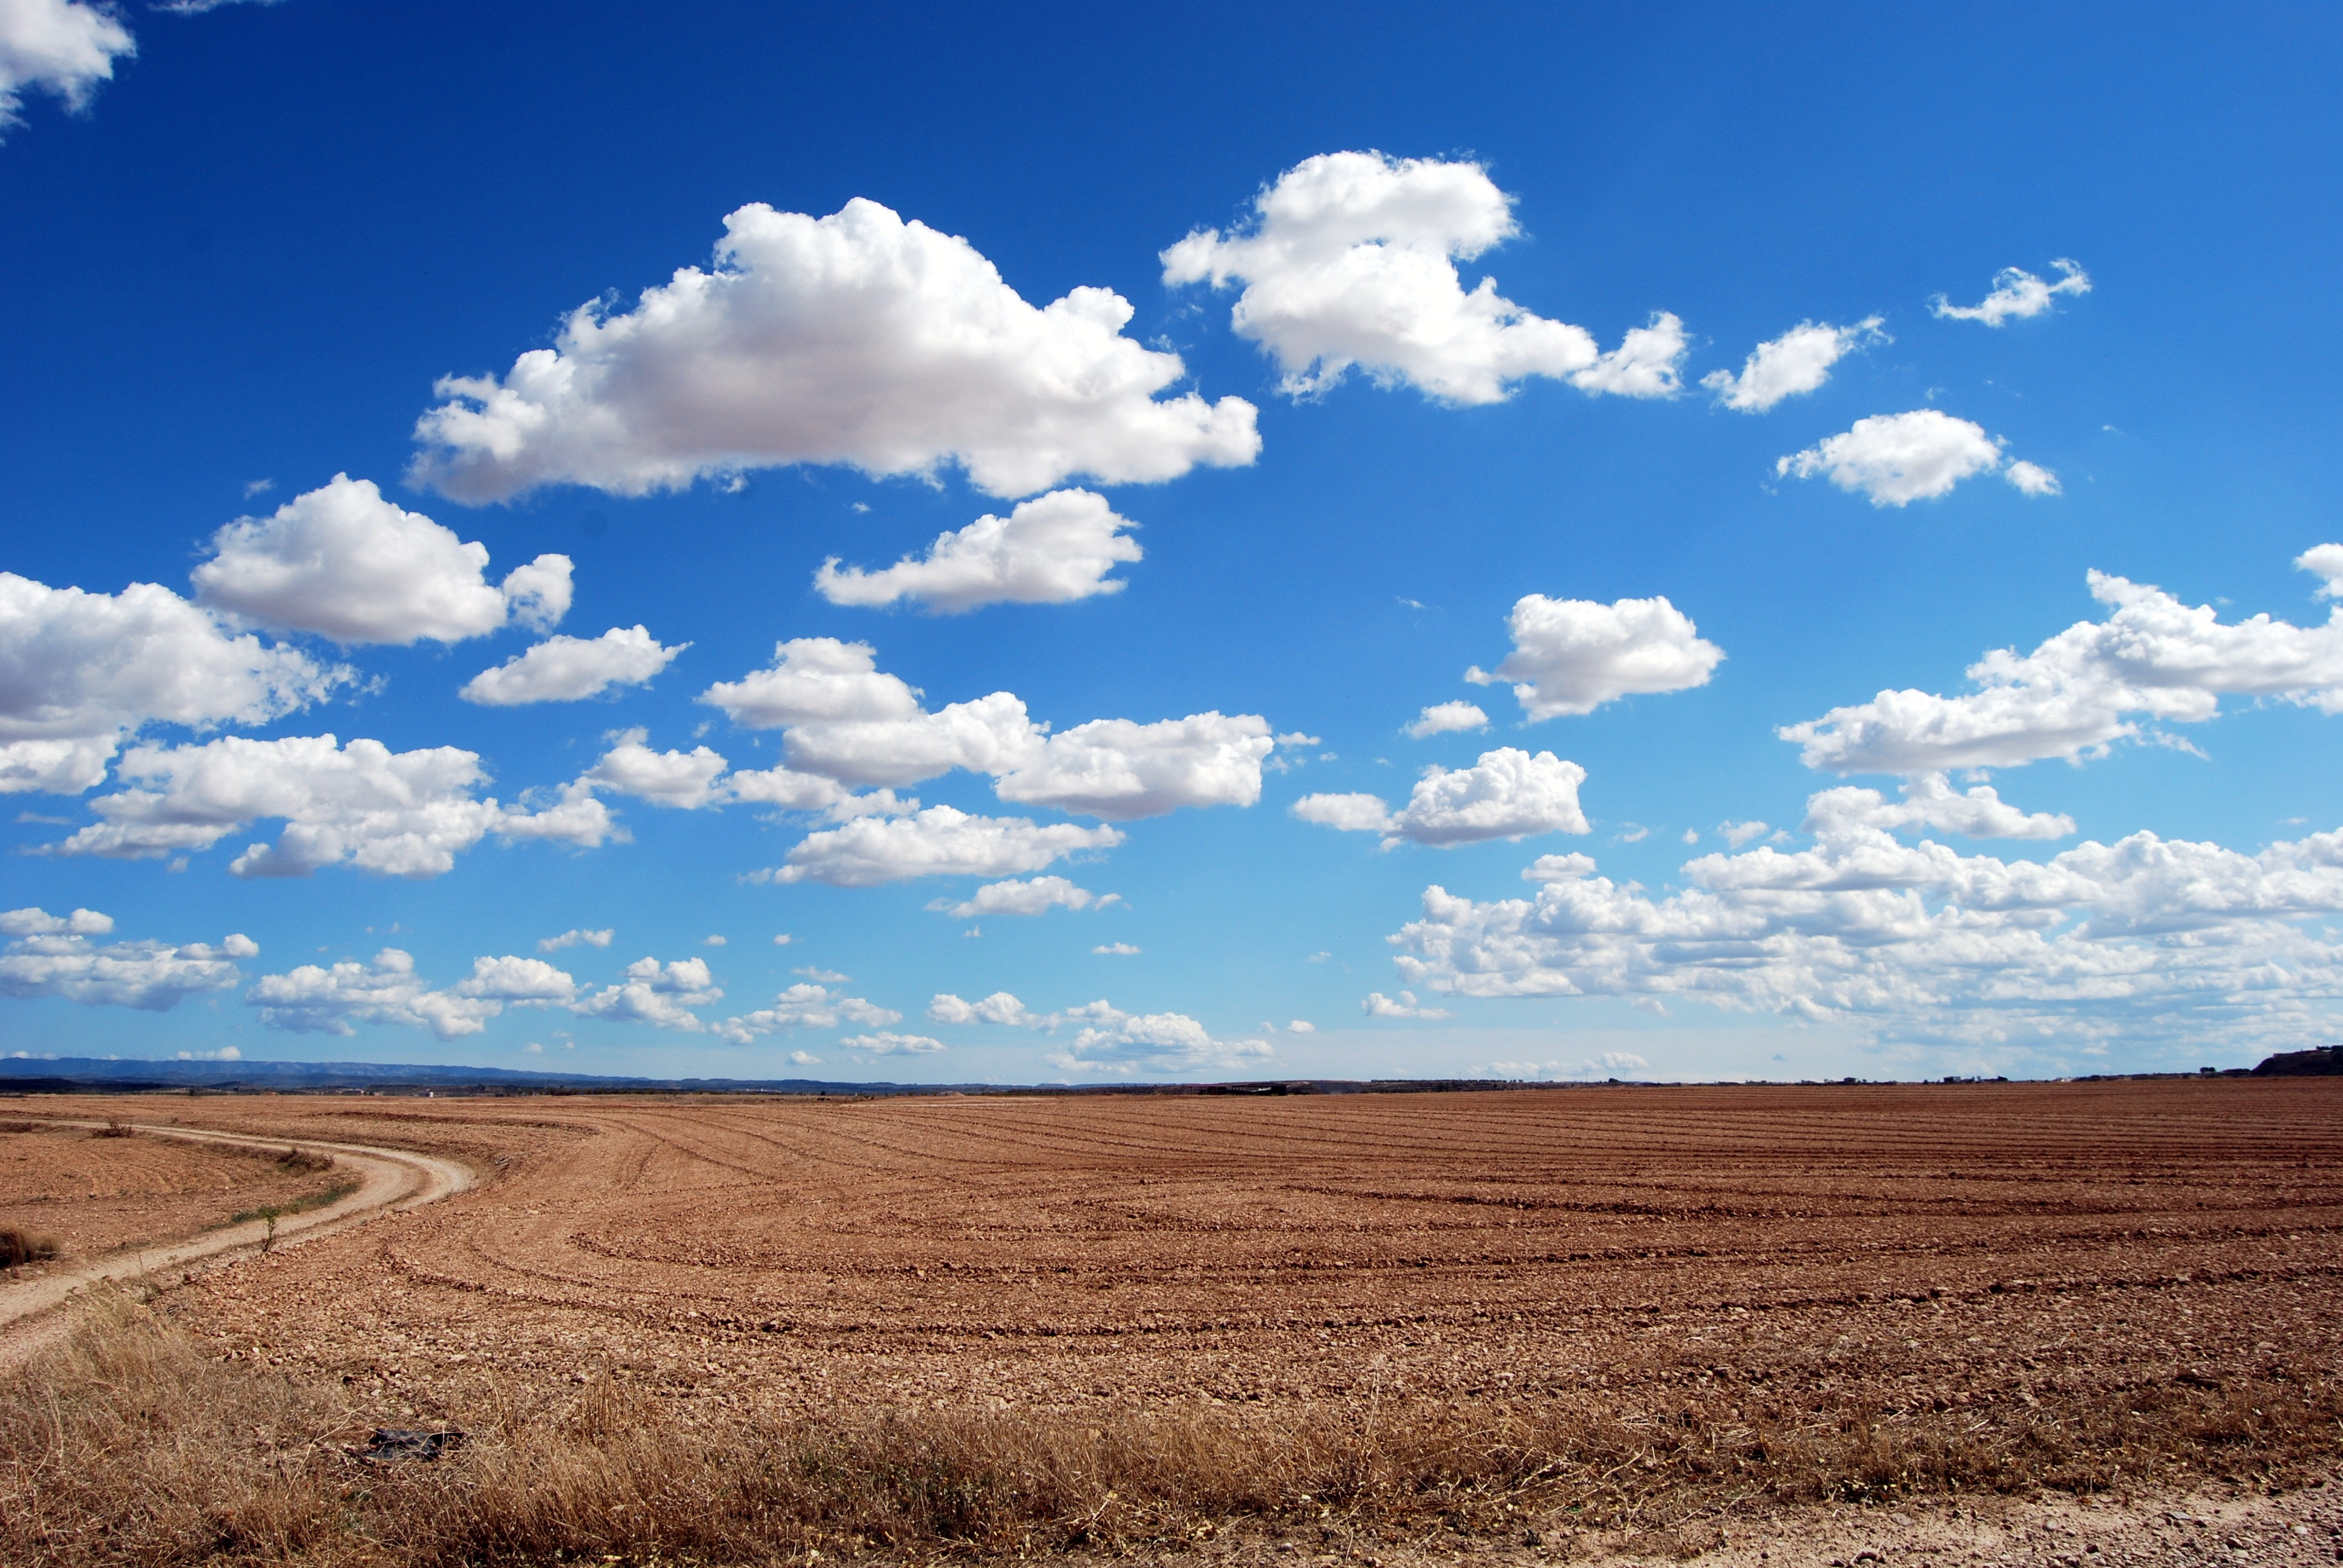
\includegraphics[width=\textwidth]{img/plains}
            \caption{Planície}
            \label{fig:plains}
        \end{subfigure}
        ~ %add desired spacing between images, e. g. ~, \quad, \qquad, \hfill etc. 
        %(or a blank line to force the subfigure onto a new line)
        \caption{Características já selecionadas}
        \label{fig:carct}
    \end{figure}
    
\end{frame}

\begin{frame}{Metodologia}
    \begin{itemize}
        \item Gerar divisões entre biomas sobre a malha de regiões;
        \item Implementar fronteiras contínuas entre biomas;
        \item Comparar resultado com cenários de jogos.
    \end{itemize}
    
    \begin{figure}[H]
        \centering
        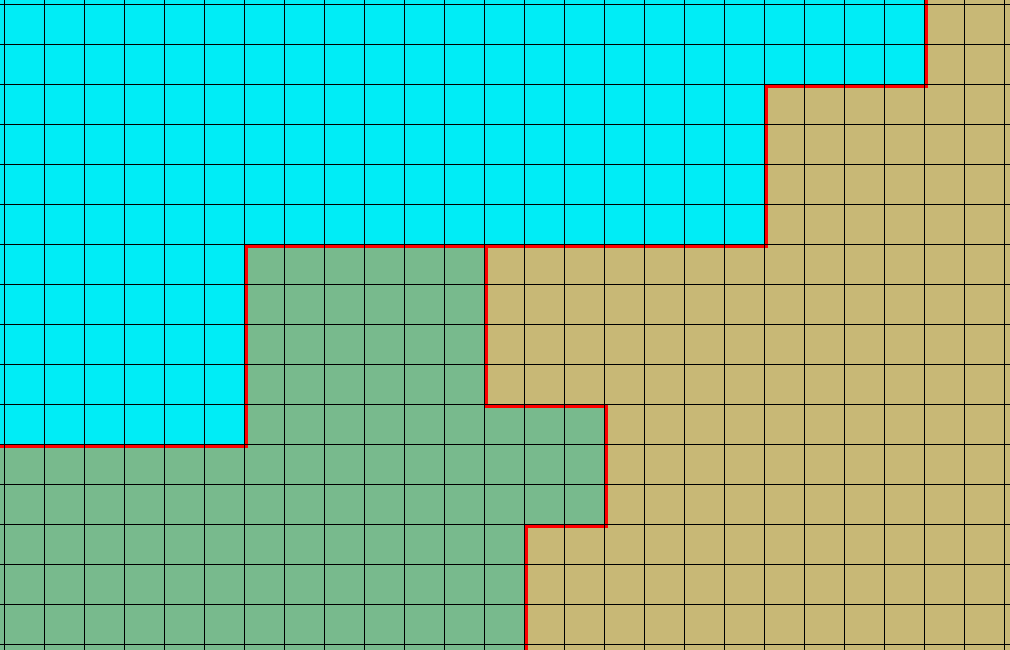
\includegraphics[width=.6\textwidth, height=.5\textheight]{img/squadStripBiomes}
        \caption{Malha com divisões de biomas.}
        \label{fig:squadStrip2}
    \end{figure}
    
\end{frame}